
\documentclass[xcolor=dvipsnames]{beamer}

\usetheme{Madrid}
\useoutertheme{miniframes} % Alternatively: miniframes, infolines, split
\useinnertheme{circles}
\usepackage{booktabs}
\usepackage[percent]{overpic}
\newcommand{\ra}[1]{\renewcommand{\arraystretch}{#1}}

\definecolor{UBCblue}{rgb}{0.04706, 0.13725, 0.26667} % UBC Blue (primary)
\definecolor{UBCgrey}{rgb}{0.0, 0.87, 0.75} % Hatsune Miku Palette (secondary) NEON 
%\definecolor{UBCgrey}{rgb}{0.0, 0.6, 0.6} % Hatsune Miku Palette (secondary)  
%\definecolor{UBCgrey}{rgb}{0.3686, 0.5255, 0.6235} % cool neon feel w UBC blue 
%\definecolor{UBCblue}{rgb}{0.04706, 0.13725, 0.26667} % UBC Blue (primary)
%\definecolor{UBCgrey}{rgb}{0.3686, 0.999, 0.6235} % UBC Grey (secondary)

\setbeamercolor{palette primary}{bg=UBCblue,fg=white}
\setbeamercolor{palette secondary}{bg=UBCblue,fg=white}
\setbeamercolor{palette tertiary}{bg=UBCblue,fg=white}
\setbeamercolor{palette quaternary}{bg=UBCblue,fg=white}
\setbeamercolor{structure}{fg=UBCblue} % itemize, enumerate, etc
\setbeamercolor{section in toc}{fg=UBCblue} % TOC sections

% Override palette coloring with secondary
\setbeamercolor{subsection in head/foot}{bg=UBCgrey,fg=white}

\usepackage{tikz}
\usetikzlibrary{calc,trees,positioning,arrows,chains,shapes.geometric,%
	decorations.pathreplacing,decorations.pathmorphing,shapes,%
	matrix,shapes.symbols}

\tikzset{
	>=stealth',
	punktchain/.style={
		rectangle, 
		rounded corners, 
		fill=black!10,
		draw=UBCblue, very thick,
		text width=10em, 
		minimum height=2em, 
		text centered, 
		on chain},
	line/.style={draw, thick, <-},
	element/.style={
		tape,
		top color=white,
		bottom color=blue!50!black!60!,
		minimum width=8em,
		draw=blue!40!black!90, very thick,
		text width=10em, 
		minimum height=3.5em, 
		text centered, 
		on chain},
	every join/.style={->, thick,shorten >=1pt},
	decoration={brace},
	tuborg/.style={decorate},
	tubnode/.style={midway, right=2pt},
}
\newcommand*\circled[1]{\tikz[baseline=(char.base)]{
		\node[shape=circle,draw,inner sep=2pt] (char) {#1};}}
		
		

\title[Meeting 2]{GDB-9 \& Small Molecule Universes}
\date{May 31, 2018}
\author[Stefan O. Gugler]
{Stefan O. Gugler}
\institute[MIT]{Massachusetts Institute of Technology  \\Department of Chemical Engineering}

\begin{document}
	
\begin{frame}
	\titlepage
\end{frame}
%
\begin{frame}
	\tableofcontents
\end{frame}

%% % % % % % % % % % % % % % % % %
%\section{Spaces and Properties}
%% % % % % % % % % % % % % % % % %
%\subsection{First Subsection}

\begin{frame}
\frametitle{Reduction of the full space}
\centering

\begin{tikzpicture}
[node distance=.5cm,
start chain=going below,]
\only<1,3->{\node[punktchain, join] (full) {Full Space};}
\only<2>{\node[punktchain, join,draw,UBCblue, ultra thick,fill=none] (full) {Full Space};}
\node[punktchain, join] (scored){Scored Space};
\node[punktchain, join] (desi){Desired Space};
\node[punktchain, join] (enum){Enumerated Space};
\node[punktchain, join] (sampl){Sample \& Build };
\visible<2>{\node[left of = desi,node distance = 6cm,rectangle,draw,UBCblue, ultra thick]  (i1) {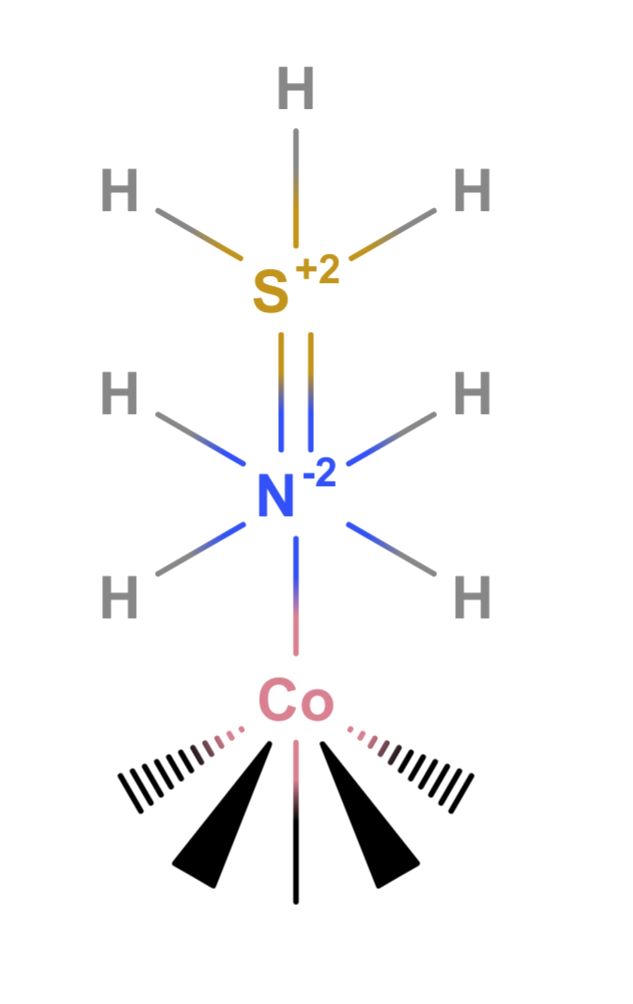
\includegraphics[width=3.5cm]{img/absurd.png}};}
\visible<2>{\path[draw,ultra thick, ->, UBCgrey] (full.west) -- (i1.east);}
\visible<3>{\node[left of = desi,node distance = 6cm]  (i2) {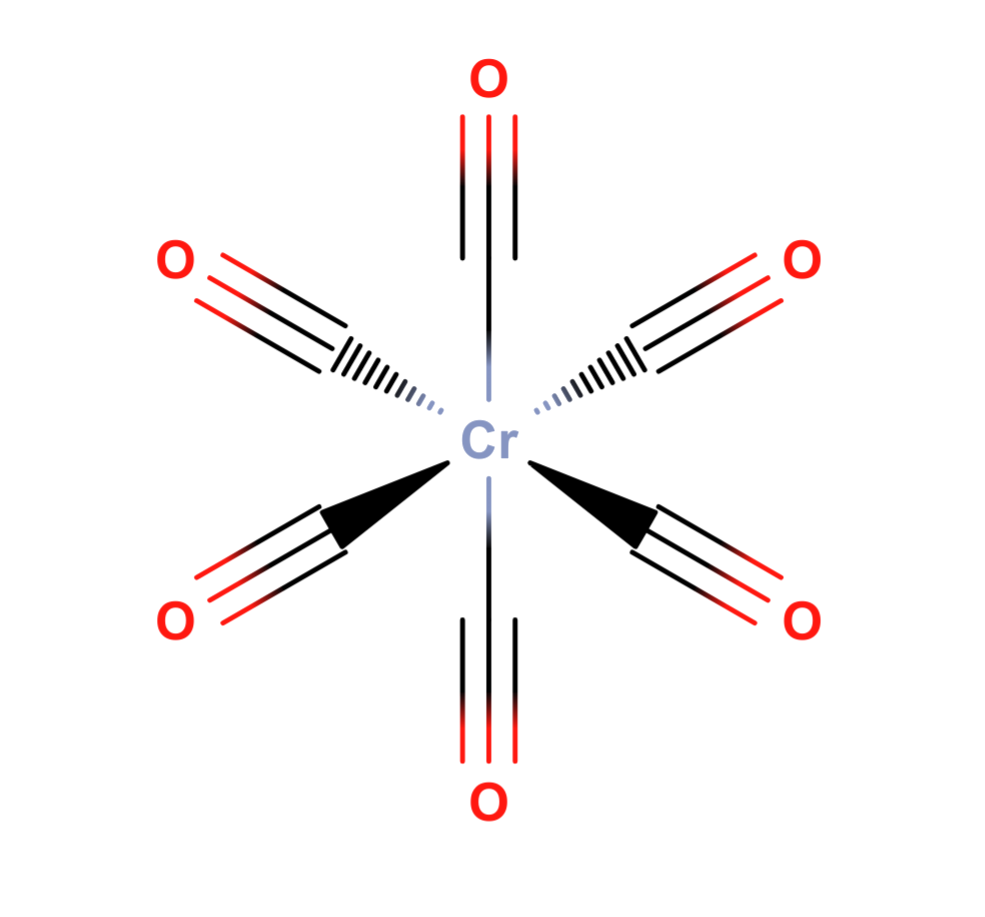
\includegraphics[width=4.5cm]{img/sensible.png}};}
\end{tikzpicture}

\end{frame}


\begin{frame}
\frametitle{Full Space $\rightarrow$ Scored Space}
% 5625 is non-trivial because different allocations of the electrons result in the same overall charge (e.g. -1/+1 == -2/+2)
\begin{itemize}
\item charge $\in [-2,+2]$
\item H atoms $\in [0,4]$
\item element $\in \textrm{\{C,~N,~O,~P,~S\}}$
\end{itemize}
~\\
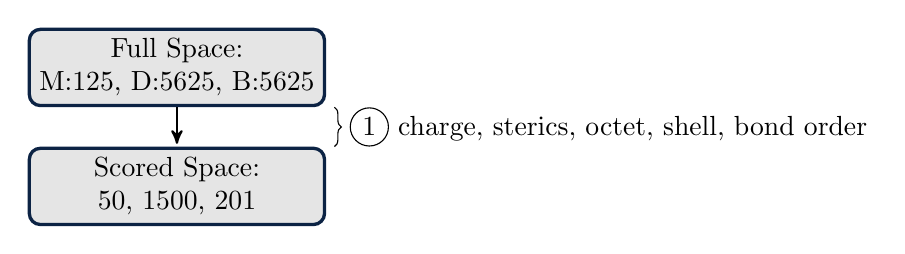
\begin{tikzpicture}
[node distance=.5cm,
start chain=going below,]
\node[punktchain, join] (full) {Full Space: \\ M:125, D:5625, B:5625};
\node[punktchain, join] (scored){Scored Space: \\ 50, 1500, 201};
\draw[tuborg, decoration={brace}] let \p1=(full.south), \p2=(scored.north) in
($(2, \y1)$) -- ($(2, \y2)$) node[tubnode] {\circled{1} charge, sterics, octet, shell, bond order};
\end{tikzpicture}
~\\
~\\
These rules \circled{1} are demonstrated in the following for the di-heavy-atoms.
\end{frame}

\begin{frame}
\frametitle{Rules \circled{1} to reduce Full Space $\rightarrow$ Scored Space}
Constraints:
\begin{itemize}
	\item Charge $c = c_1 + c_2 \leq 1 $
	\item Sterics: H atoms $<$ 4 on connecting atoms
	\item Closed shell (even number of electrons)
\end{itemize}
~\\
~\\
$\rightarrow$ Reduces 5625 ligands to 1171.
\end{frame}


\begin{frame}
\frametitle{Rules \circled{1} to reduce Full Space $\rightarrow$ Scored Space}
\begin{equation}
u_{\textrm{octet,i}} = 
\begin{cases}
10 + 2 \cdot (8-VE_i) 	& \mathrm{if}~ 8-VE_i < 0 \\
10 - 1 \cdot (8-VE_i) 	& \mathrm{if}~ 8-VE_i \geq 0
\end{cases}
\end{equation}

\begin{equation}
u_{\textrm{charge}} = 
\begin{cases}
0	&	\mathrm{if}~ c_1 + c_2 > 0 \\
3	&	\mathrm{if}~ 0 \geq c_1 + c_2 \geq -2 \\
1   &	\mathrm{if}~ c_1 + c_2 = -3 \\
0   &	\mathrm{if}~ c_1 + c_2 = -4 
\end{cases}
\end{equation}

\begin{equation}
u_{\textrm{VSEPR}} = 
 5-|\underbrace{(VE_1 - 2 \cdot LP_1 + c_1 - 2 \cdot h_1)}_{ready~electrons} -  \underbrace{(VE_2 - 2 \cdot LP_2 + c_2 - 2 \cdot h_2)}_{ready~electrons}|
\end{equation}
\end{frame}

\begin{frame}
\frametitle{Rules \circled{1} to reduce Full Space $\rightarrow$ Scored Space}

\begin{equation}
u_{\textrm{CA}} = 
\begin{cases}
1	&	\mathrm{if}~ h_1 = 4 \\
2	&	\mathrm{if}~ h_1 = 3 \\
3   &	\mathrm{if}~ \textrm{else} 
\end{cases}
\end{equation}

\begin{equation}
u_{\textrm{shell}} = 
\begin{cases}
1	&	\mathrm{if}~ \neg (VE_1+VE_2) \% 2 \\
0	&	\mathrm{if}~ \textrm{else}
\end{cases}
\end{equation}

\begin{equation}
u_{\textrm{total}} = u_{\textrm{shell}} \cdot \left( \frac{1}{2} ( u_{\textrm{octet,1}} + u_{\textrm{octet,2}} ) + u_{\textrm{charge}} + u_{\textrm{VSEPR}} + u_{\textrm{CA}} \right)
\end{equation}

where $VE_i$ denotes the number of valence electrons, $LP_i$ the number of lone pairs.
\end{frame}

\begin{frame}
\frametitle{Distribution and Examples}
\centering
\begin{overpic}[width=0.8\linewidth]{img/distrDiCNOPS.pdf}
	\put (13,24) {[C--]=[OH2--]}
	\put (15,31) {[N--]-[PH4--]}
	\put (25,37) {[CH3]-[SH2-]}
	\put (30,45) {[PH++]\#0[SH3-]}
	
	\put (56,53) {[NH2]-[OH]}
	\put (80,57) {[C+]\#[O-]}
	\put (78,51) {[O-]\#[O-]}
\end{overpic}
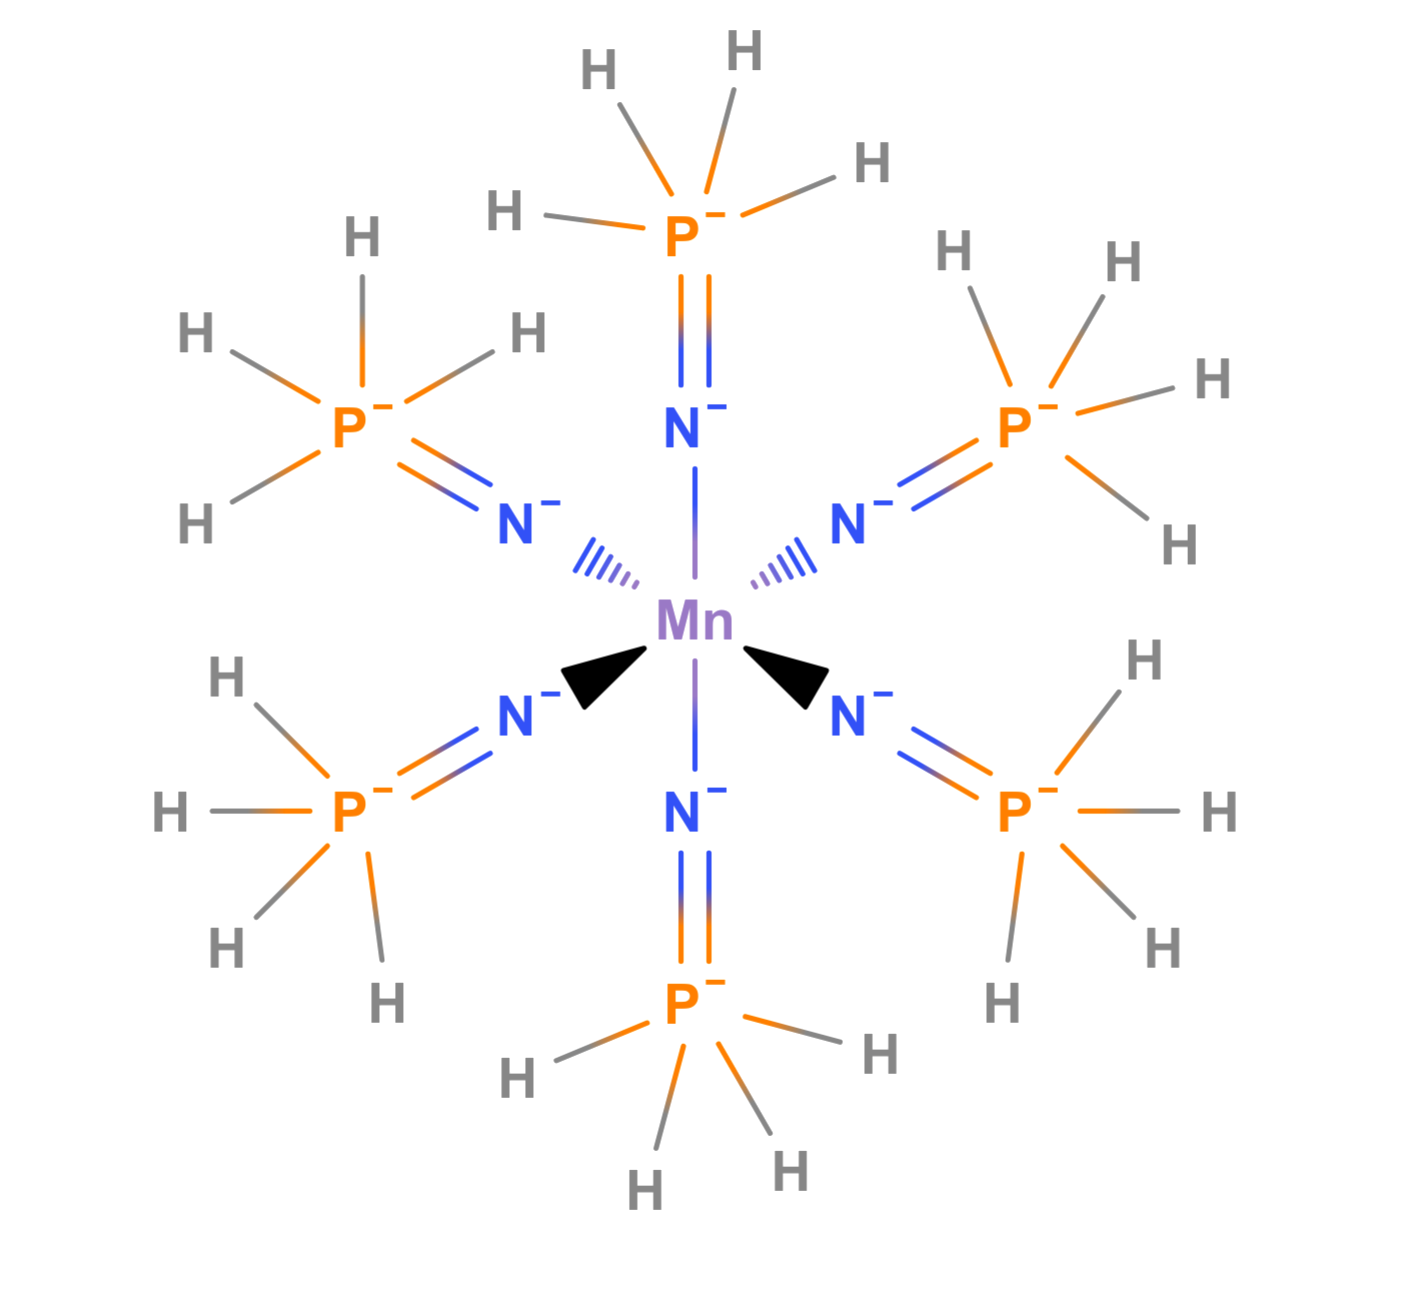
\includegraphics[width=3.5cm]{img/evenlesssens.png}
\end{frame}

\begin{frame}
\frametitle{Reduction of the full small ligand universe: Mo, Di, Bi}

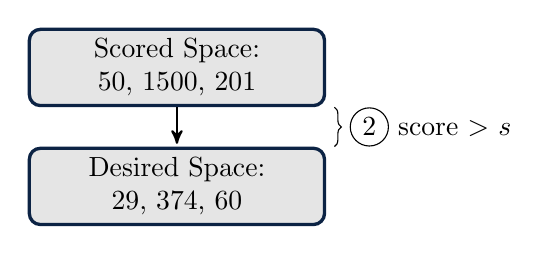
\begin{tikzpicture}
[node distance=.5cm,
start chain=going below,]
\node[punktchain, join] (scored){Scored Space: \\ 50, 1500, 201};
\node[punktchain, join] (desi){Desired Space: \\ 29, 374, 60};

\draw[tuborg] let \p1=(scored.south), \p2=(desi.north) in
($(2, \y1)$) -- ($(2, \y2)$) node[tubnode] {\circled{2} score $>$ $s$};
\end{tikzpicture}


\end{frame}

\begin{frame}
\frametitle{Reduction of the full small ligand universe: Mo, Di, Bi}

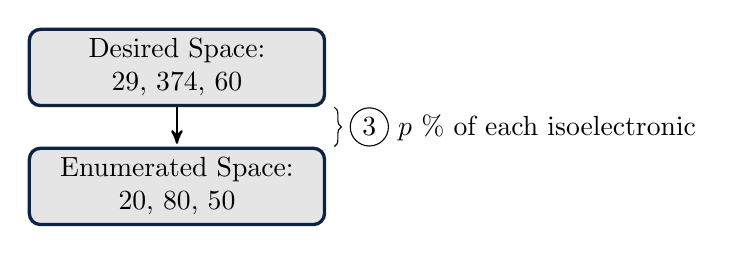
\begin{tikzpicture}
[node distance=.5cm,
start chain=going below,]
\node[punktchain, join] (desi){Desired Space: \\ 29, 374, 60};
\node[punktchain, join] (enum){Enumerated Space: \\ 20, 80, 50};

\draw[tuborg] let \p1=(desi.south), \p2=(enum.north) in
($(2, \y1)$) -- ($(2, \y2)$) node[tubnode] {\circled{3} $p$ \% of each isoelectronic};
\end{tikzpicture}
\end{frame}

\begin{frame}
\frametitle{Reduction of the full small ligand universe: Mo, Di, Bi}

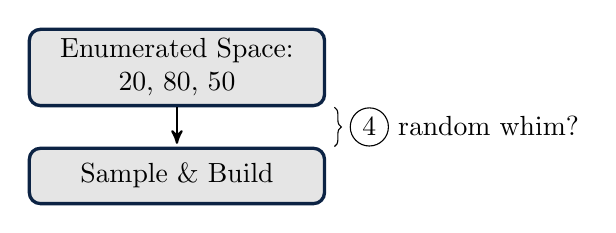
\begin{tikzpicture}
[node distance=.5cm,
start chain=going below,]
\node[punktchain, join] (enum){Enumerated Space: \\ 20, 80, 50};
\node[punktchain, join] (sampl){Sample \& Build };

\draw[tuborg] let \p1=(enum.south), \p2=(sampl.north) in
($(2, \y1)$) -- ($(2, \y2)$) node[tubnode] {\circled{4} random whim?};
\end{tikzpicture}
\end{frame}



\begin{frame}
\frametitle{Subsets of octahedral space}
The sizes of the selected subsets of octahedral space.
\begin{table}[]
	\centering
%	\caption{The sizes of the selected subsets of octahedral space.}
	\label{tab:space-sizes}
	\begin{tabular}{llr}
		\toprule
		Set 					& description		    	   & size \\
		\midrule
		Homoleptics             & eq = ax                   & 553        \\[0.1cm]
		"5+1" symmetric         & eq = ax1 $\neq$ ax2       & 163,620    \\[0.1cm]
		"4+2" symmetric         & eq1 $\neq$ eq2 = ax       & 185,376    \\[0.1cm]
		Strongly symmetric      & eq $\neq$ ax              & 245,316    \\[0.1cm]
		Equatorially asymmetric & eq1 $\neq$ eq2 $\neq$ ax  & 15,924,796 \\[0.1cm]
		Weakly symmetric        & eq $\neq$ ax1 $\neq$ ax2  & 45,077,310 \\[0.1cm]
		Complete Heteroleptics  & $L_i \neq L_j$            & $\approx 5.9 \cdot 10^{12}$ \\[0.1cm] %405!/399!/6!+148!/145!/3!
		Octahedral Space        & all                       & $> 1.8 \cdot 10^{14}$ \\
		%number of cube colorings as lower bound
		\bottomrule
	\end{tabular}
	\end{table}
\end{frame}


\begin{frame}
\frametitle{Properties of the sets}
\begin{itemize}
\item Reduce space to facilitate sampling from non-homoleptics
\item Example: strongly symmetric, monodentate ligand fields (163,620)
\item Exclude all with charge smaller than -4, which results in 87,150 ligand fields (53~\%).
\end{itemize}

\begin{figure}[ht] 
	\begin{minipage}[b]{0.5\linewidth}
		\centering
		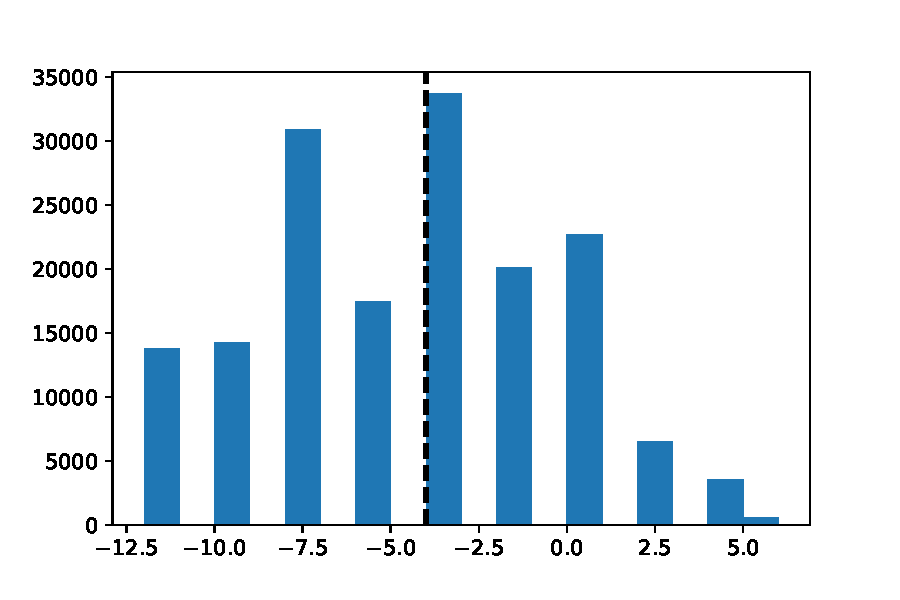
\includegraphics[width=.8\linewidth]{img/strongsymMonodentates_chargeHist.pdf} 
		\vspace{4ex}
	\end{minipage}%%
	\begin{minipage}[b]{0.5\linewidth}
		\centering
		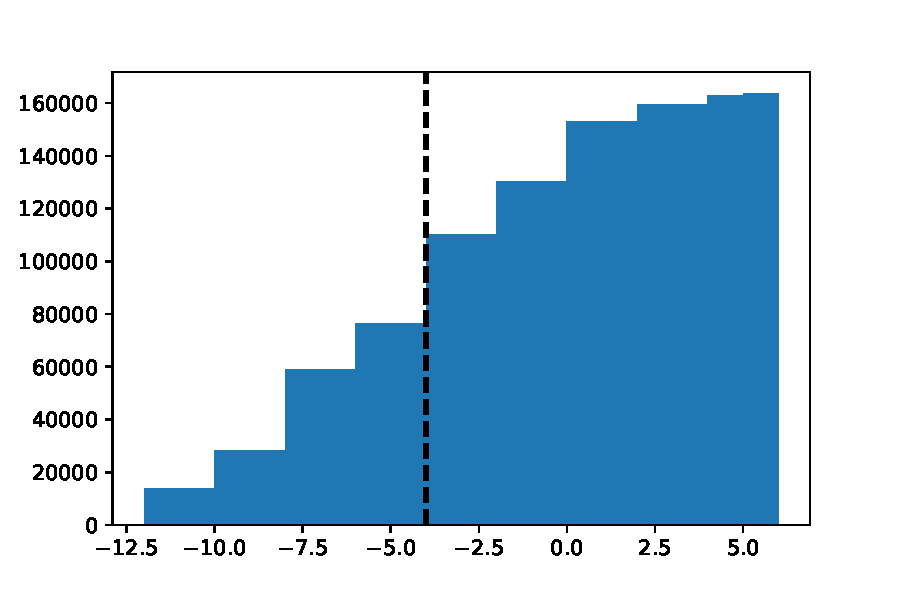
\includegraphics[width=.8\linewidth]{img/strongsymMonodentates_chargeHistCum.pdf} 
		\vspace{4ex}
	\end{minipage} 
\end{figure}
\end{frame}


\begin{frame}
\frametitle{Principal Component Analysis}
The homoleptics (ho) span the strong symmetry (ss) and "5+1" (fo) set.
\begin{figure}
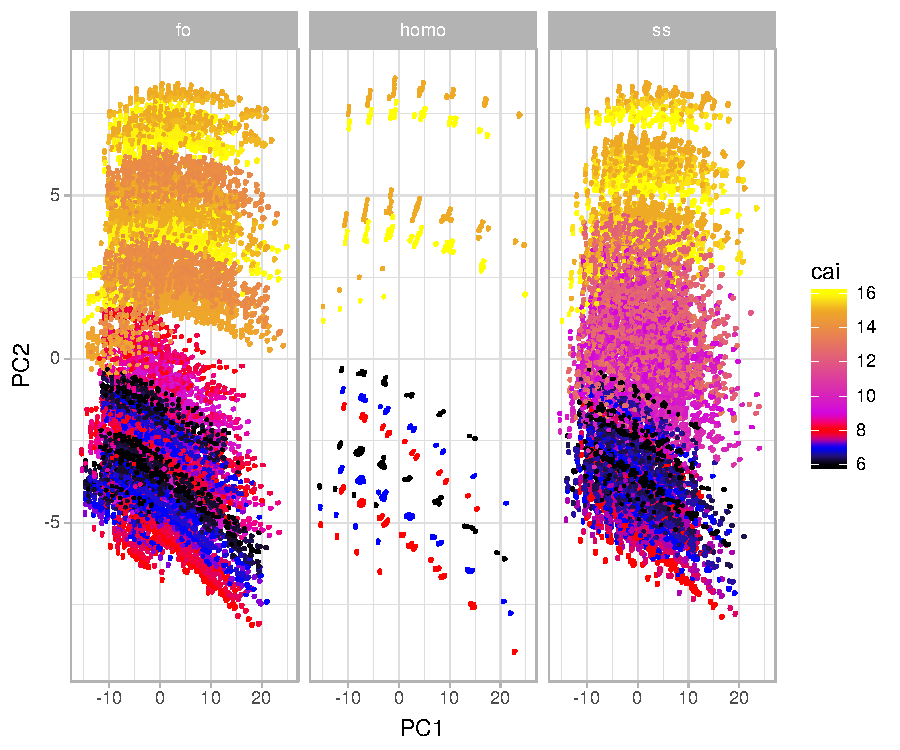
\includegraphics[width=0.65\linewidth]{img/pca.pdf}
\caption{asd} 
\end{figure}
\end{frame}

\begin{frame}
	\frametitle{Footprint and Entropy calculation}
	We use five properties to characterize the ligand field and generate a five dimensional distribution:
	\begin{itemize}
	\item total charge
	\item total valence electrons
	\item electronegativity of the connecting atom
	\item $^{\textrm{lc}}_{\textrm{ax,eq}}\chi_1 = \sum{EN_{\textrm{CA}} \cdot EN_i}$
	\item $^{\textrm{lc}}_{\textrm{ax,eq}}\chi^\prime_1 = \sum{EN_{\textrm{CA}} - EN_i}$
	
	\end{itemize}
	We then calculate the entropy, $H_{\textrm{KDE}}$, of the Kernel Density Estimated distrbution.
\end{frame}

\begin{frame}
\frametitle{Correlation analysis for strongly symmetric monodentates }
\begin{figure}
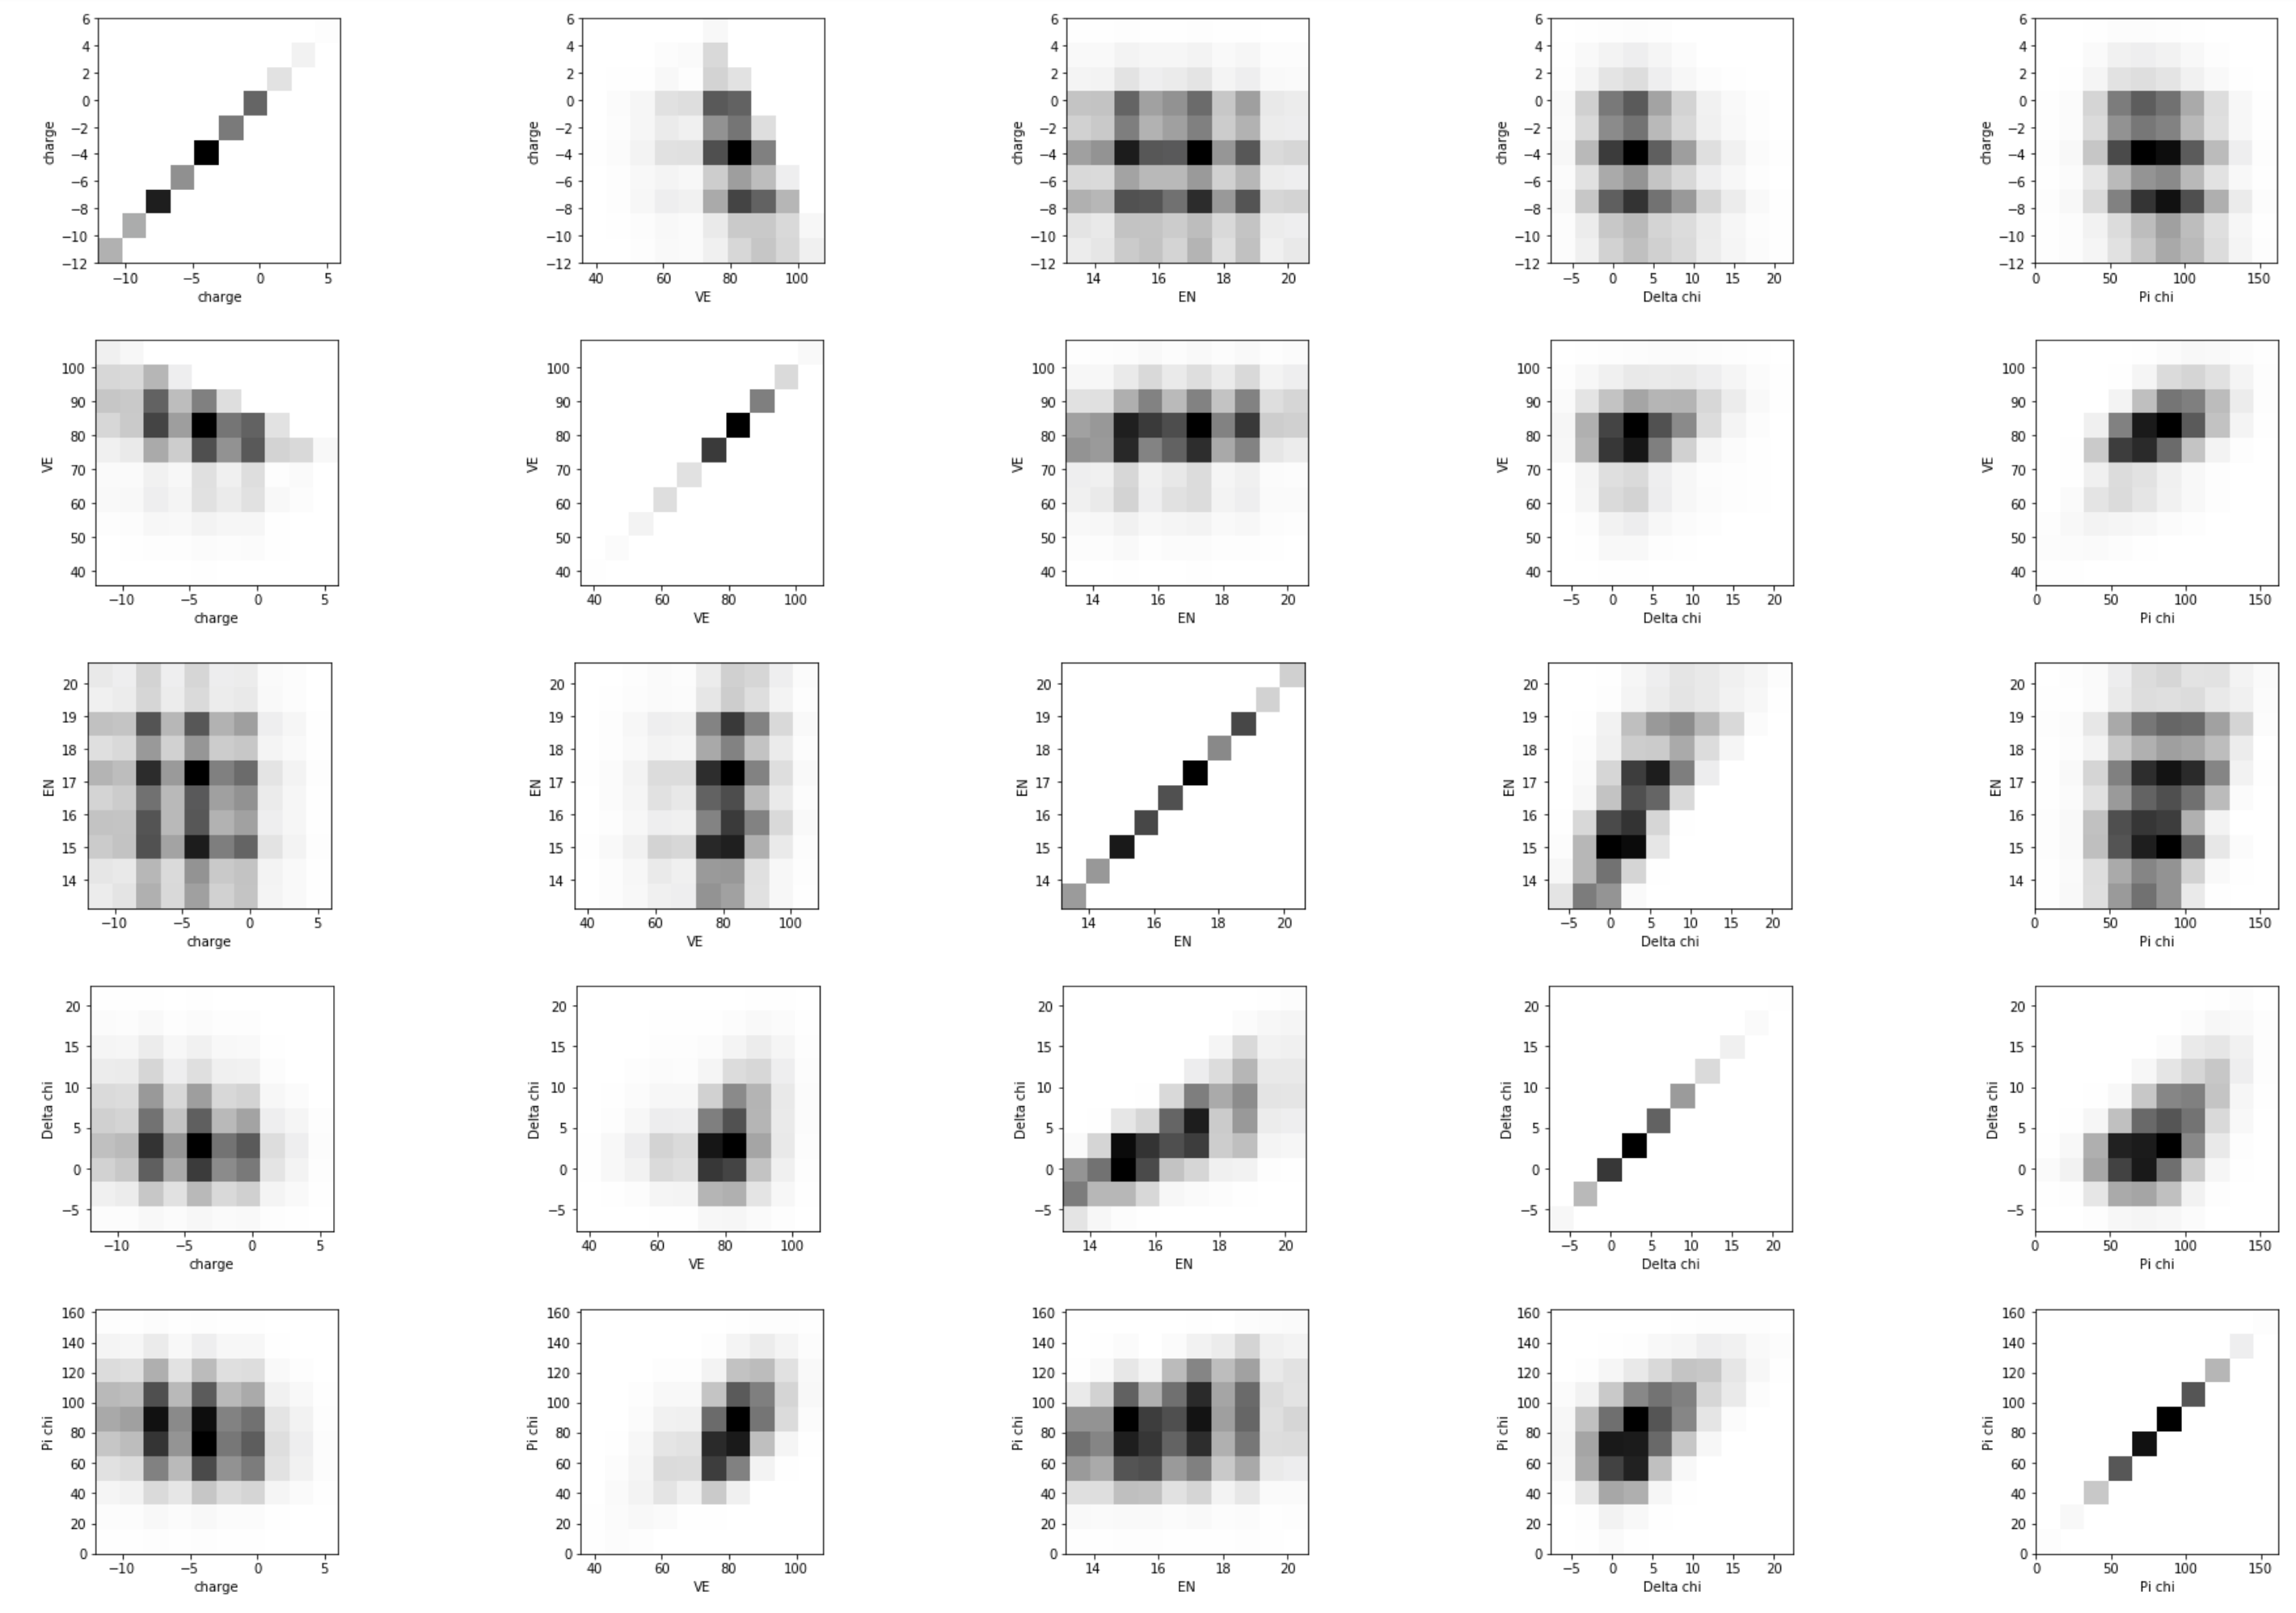
\includegraphics[width=0.65\linewidth]{img/strongsymMonodentates_PairwiseCorr.png}
\end{figure}
\centering
\end{frame}

\begin{frame}
\frametitle{Example of KDE slice}
Dimensions $^{\textrm{lc}}_{\textrm{ax,eq}}\chi_1$ vs. charge in $H_{\textrm{KDE}}$ for strongly symmetric monodentates.
\begin{figure}[ht] 
	\begin{minipage}[b]{0.5\linewidth}
		\centering
		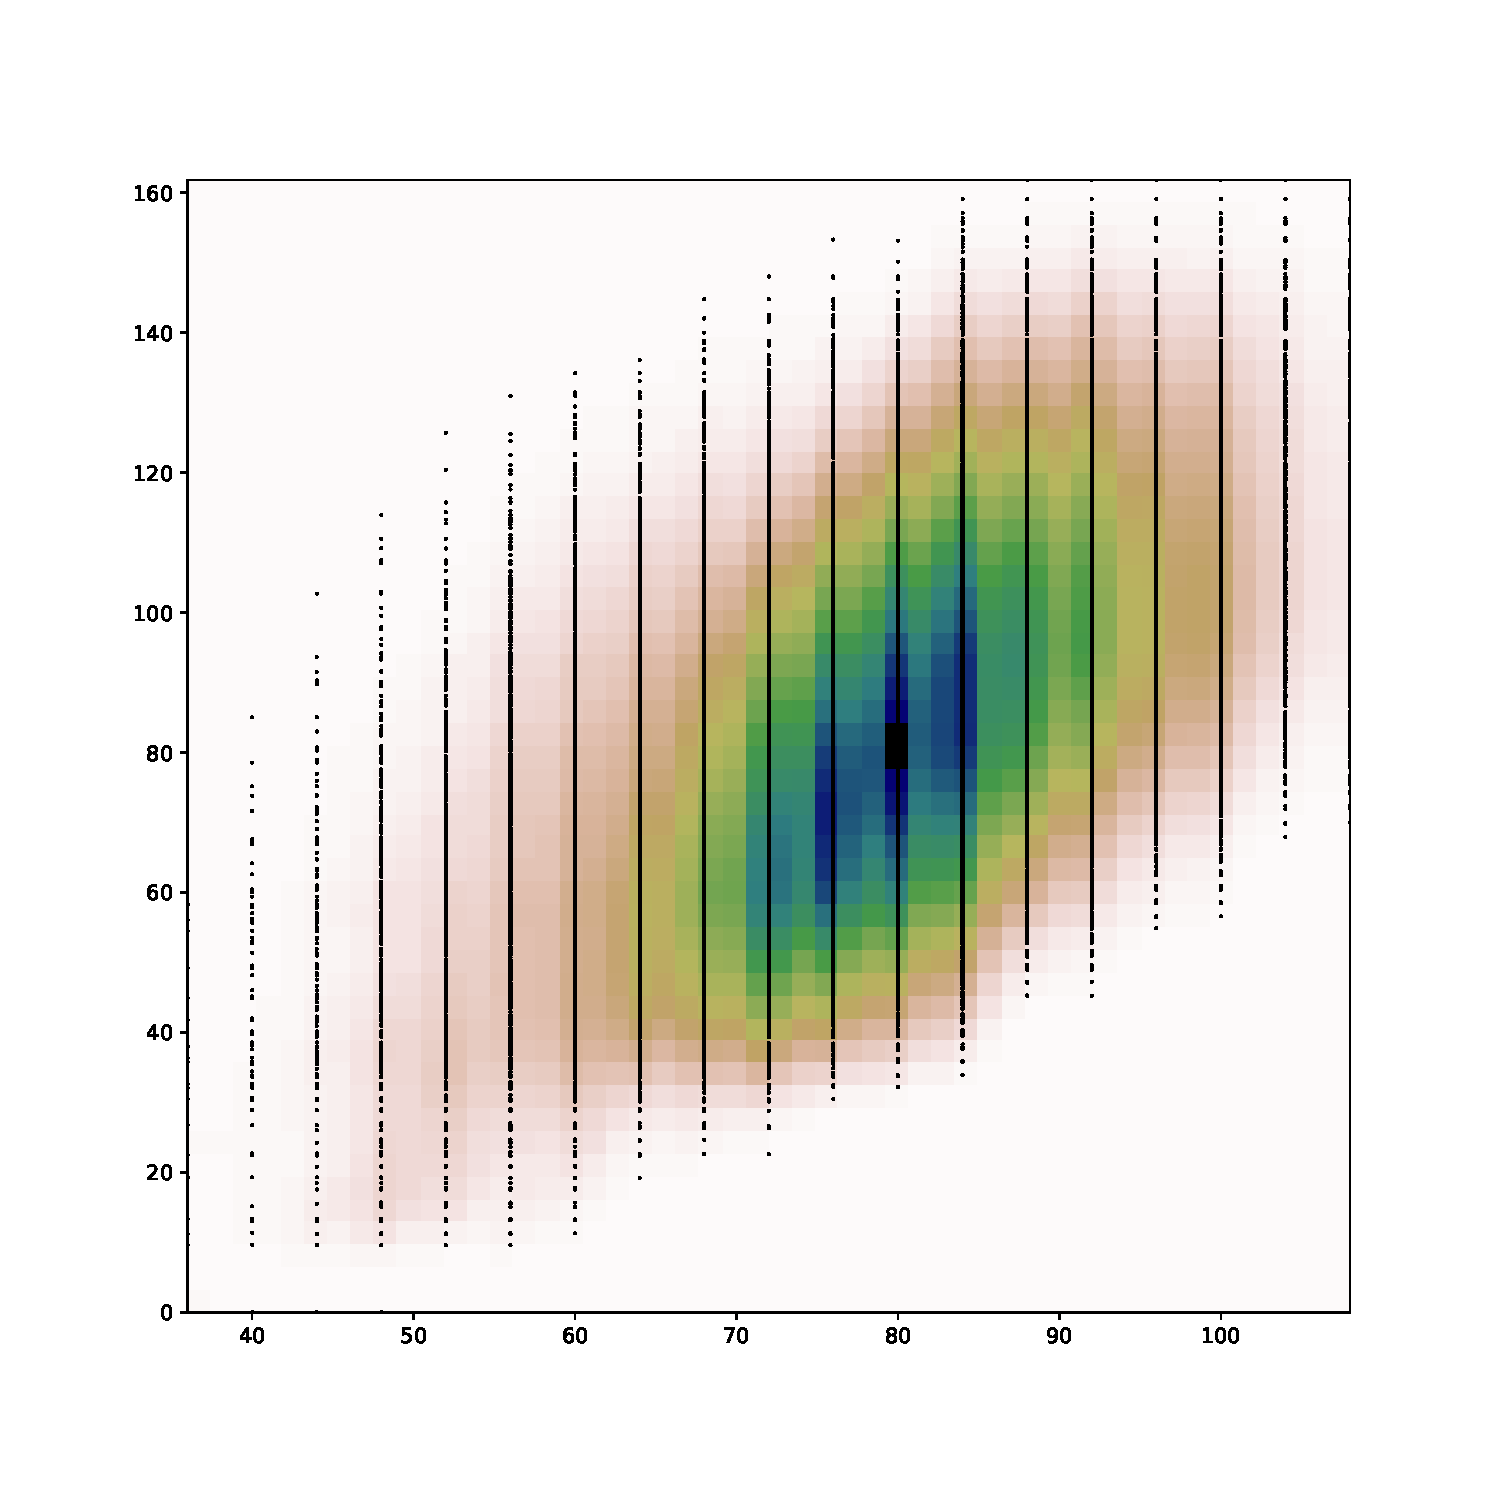
\includegraphics[width=1\linewidth]{img/strongsymMonodentates_heatmap.pdf} 
		\vspace{2ex}
	\end{minipage}%%
	\begin{minipage}[b]{0.5\linewidth}
		\centering
		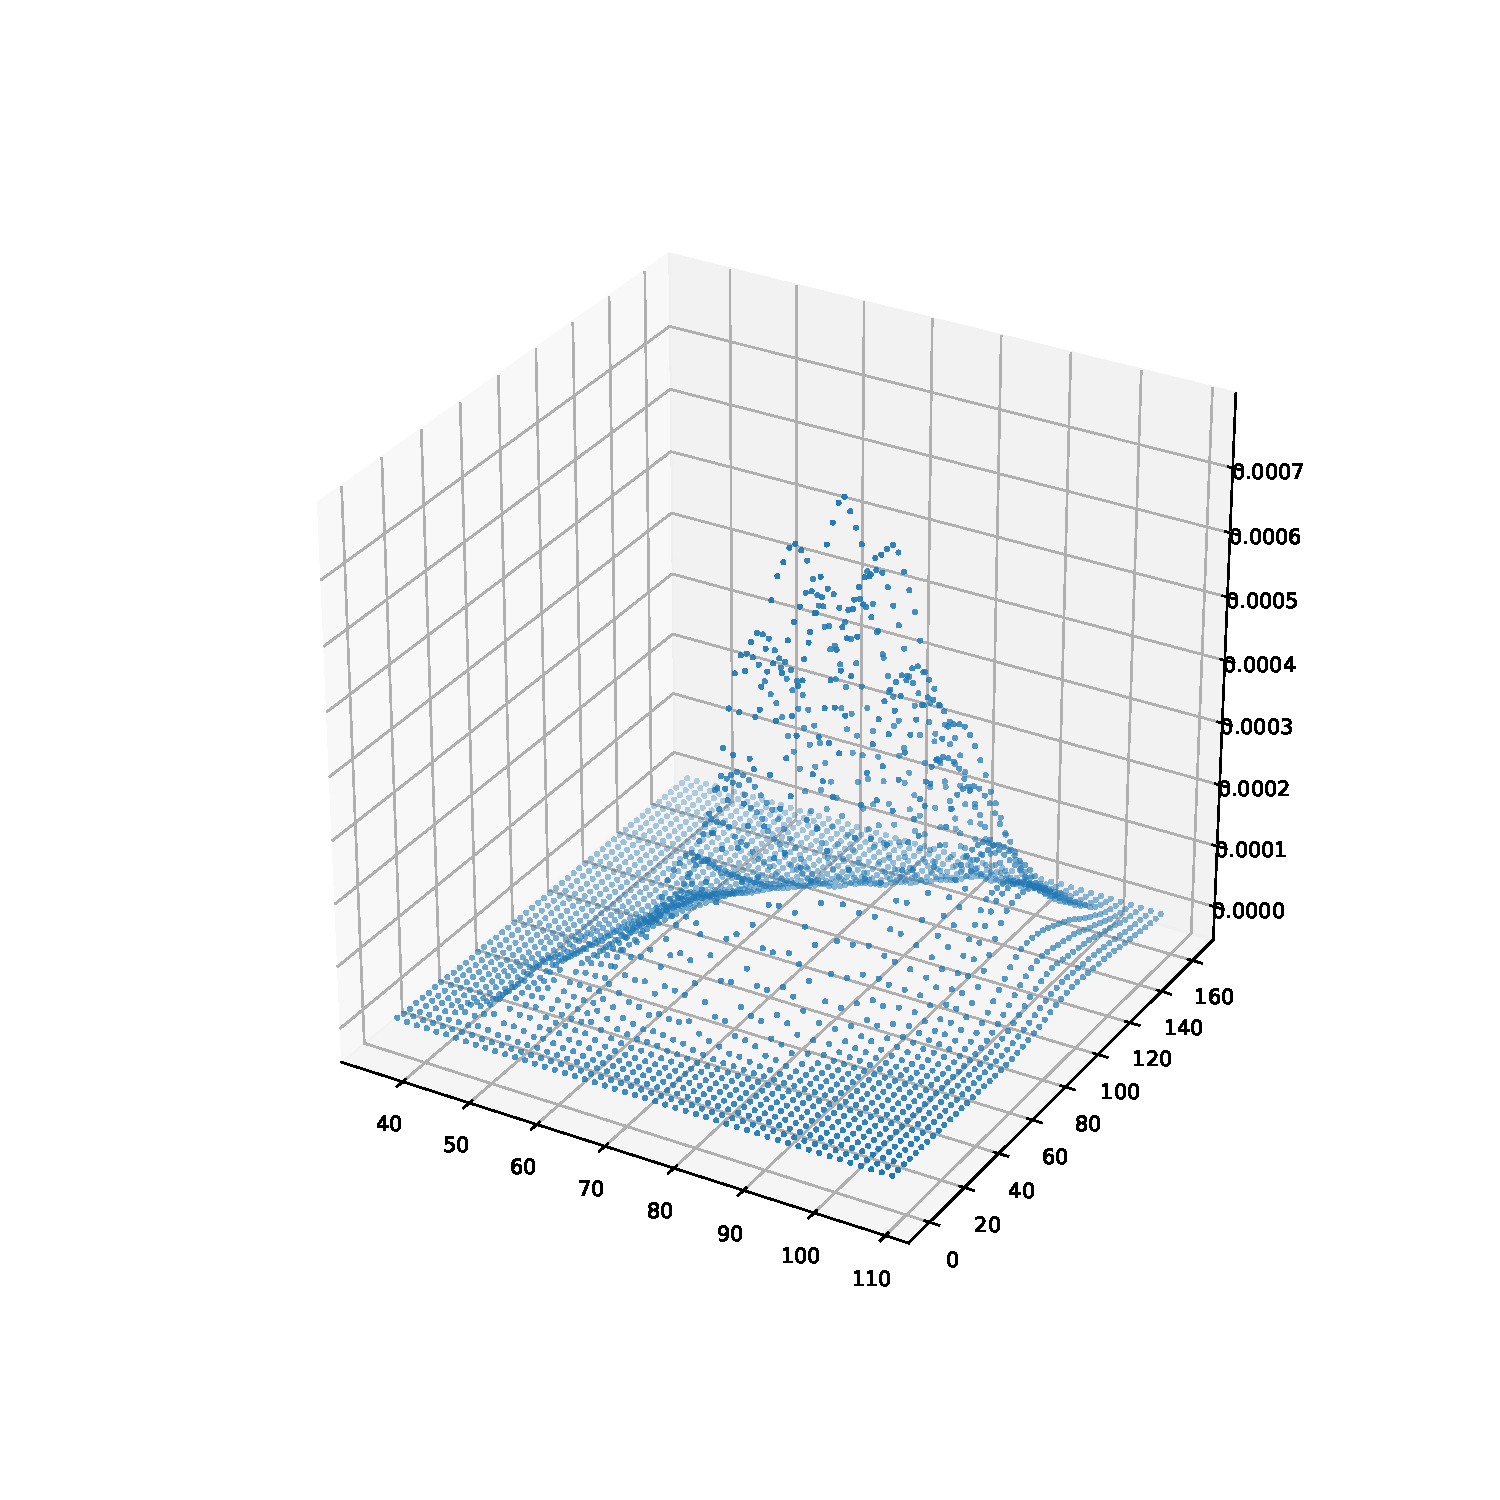
\includegraphics[width=1\linewidth]{img/strongsymMonodentates_3Dhists.pdf} 
		\vspace{2ex}
	\end{minipage} 
\end{figure}
\end{frame}

\begin{frame}
\frametitle{Monodentate Footprints}
	\begin{table}[]
	\centering
	\caption{Entropic footprint}
	\label{tab:ent-footprint}
	\begin{tabular}{lcr}
		\toprule
		Set 					    &  $H_{\textrm{KDE}}^{\textrm{monodent}}$   & $H_{\textrm{KDE}}^{\textrm{bident}}$ \\
		\midrule
		Homoleptics                 &  19.7  & 15.63   \\[0.1cm]
		"5+1" symmetric             &  13.7  & -       \\[0.1cm]
		Strongly symmetric AC       &  -     & 9.47    \\[0.1cm]
		Strongly symmetric ADC      &  12.70 & 5.53    \\[0.1cm]
		"4+2" symmetric             &  12.70 & 9.47    \\[0.1cm] 
		Weakly symmetric            &  8.1   & 7.7     \\[0.1cm]
		Equatorially asymmetric AC  &  -     & 10.04   \\[0.1cm]
		Equatorially asymmetric ADC &        &         \\[0.1cm]

		\bottomrule
	\end{tabular}
	\end{table}
\end{frame}

\begin{frame}
\frametitle{Entropy histogram}
\begin{figure}
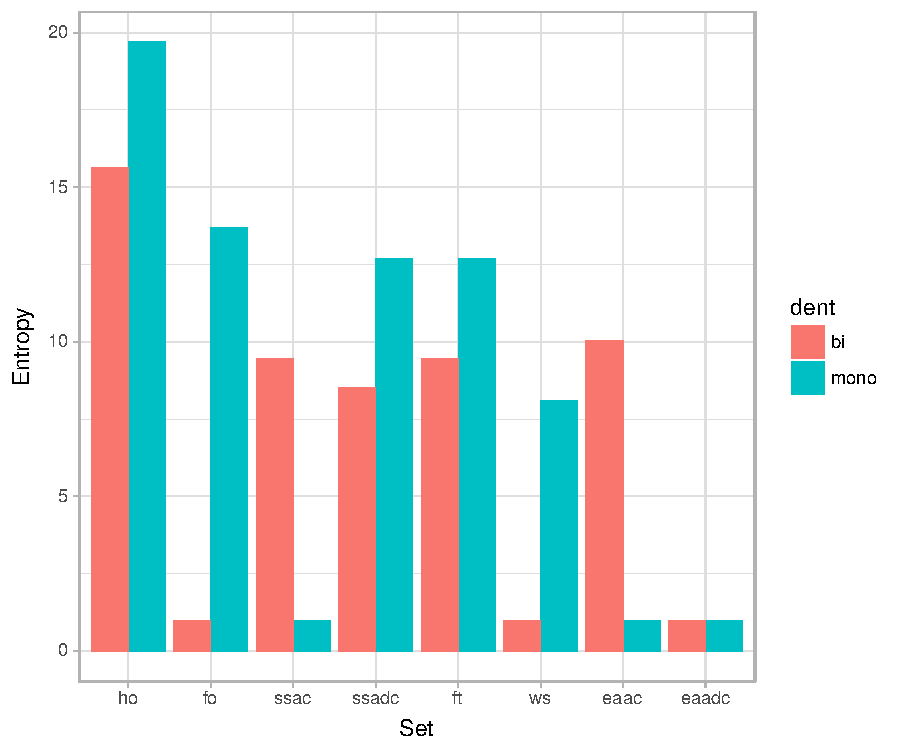
\includegraphics[width=0.7\linewidth]{img/ent.pdf}
\end{figure}
\end{frame}

%
%\begin{frame}
%\frametitle{Actual calculations}
%The calculations, colored by convergence fitness.
%\begin{figure}
%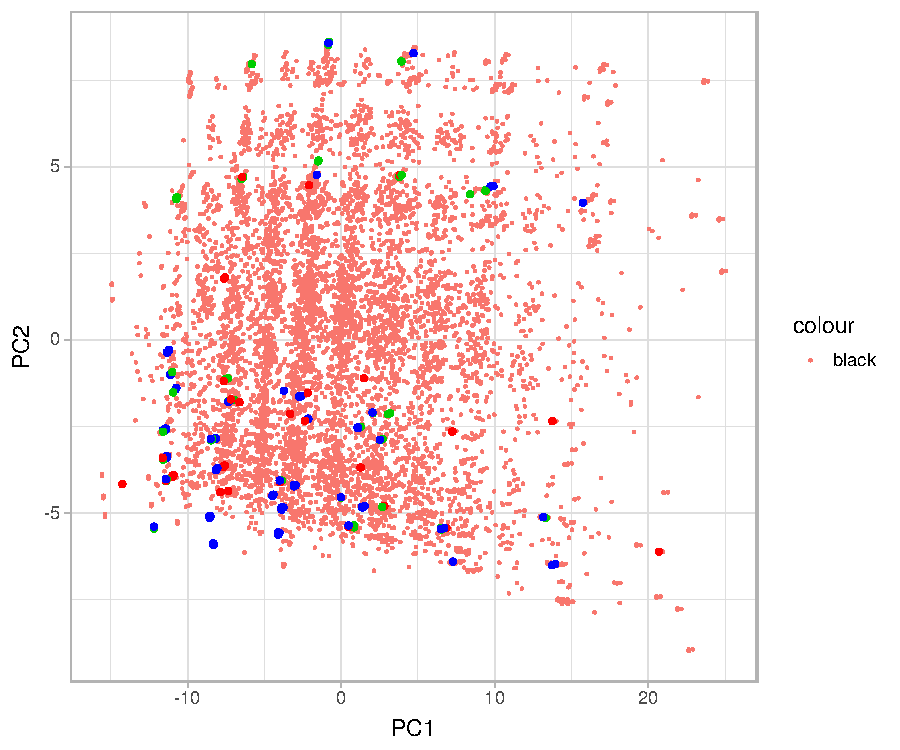
\includegraphics[width=0.7\linewidth]{img/pcaWithCalcs.pdf}
%\end{figure}
%\end{frame}

\begin{frame}
\frametitle{Actual calculations}
\begin{figure}[ht] 
	\label{ fig7} 
	\begin{minipage}[b]{0.5\linewidth}
		\centering
		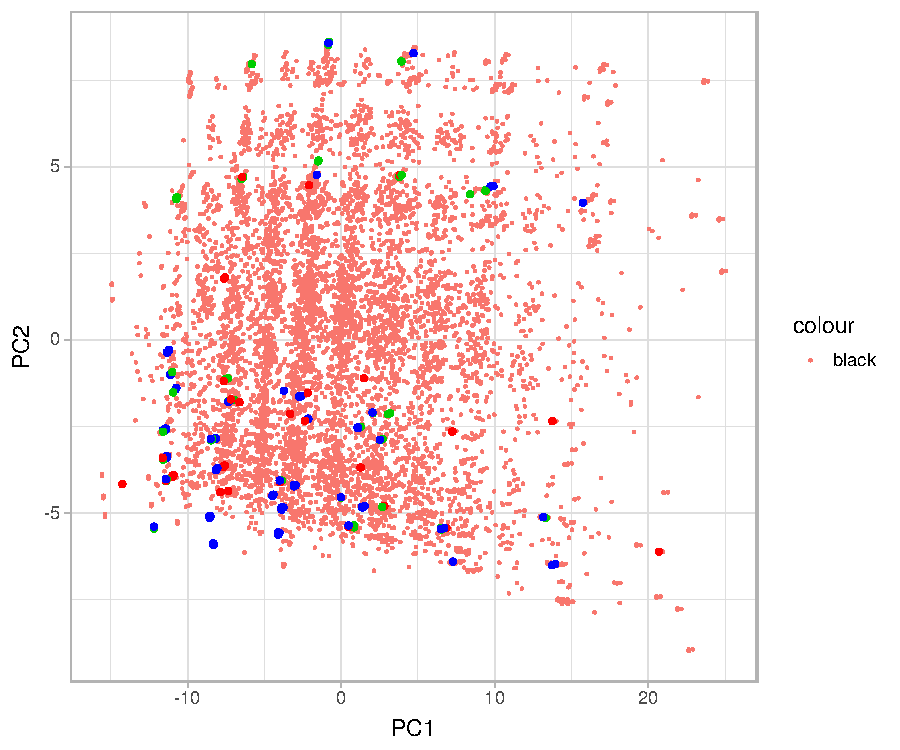
\includegraphics[width=.6\linewidth]{img/pcaWithCalcs.pdf} 
%		\vspace{8ex}
	\end{minipage}%%
	\begin{minipage}[b]{0.5\linewidth}
		\centering
		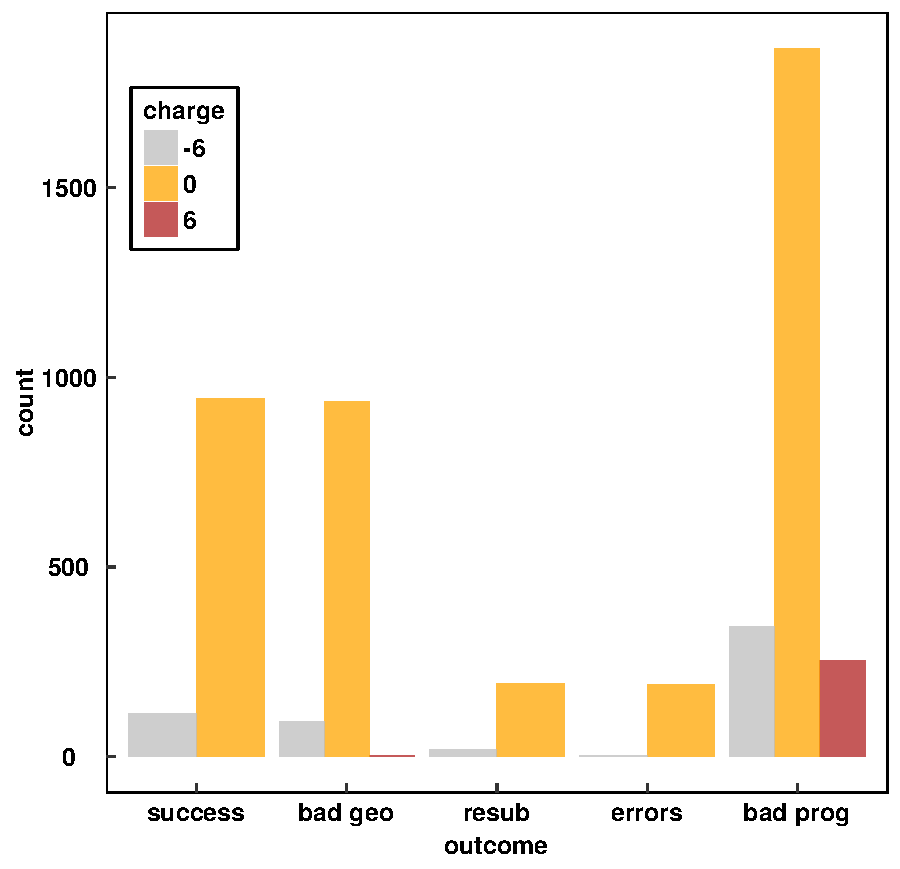
\includegraphics[width=.6\linewidth]{img/fateByCharge.pdf} 
%		\vspace{8ex}
	\end{minipage} 
	\begin{minipage}[b]{0.5\linewidth}
		\centering
		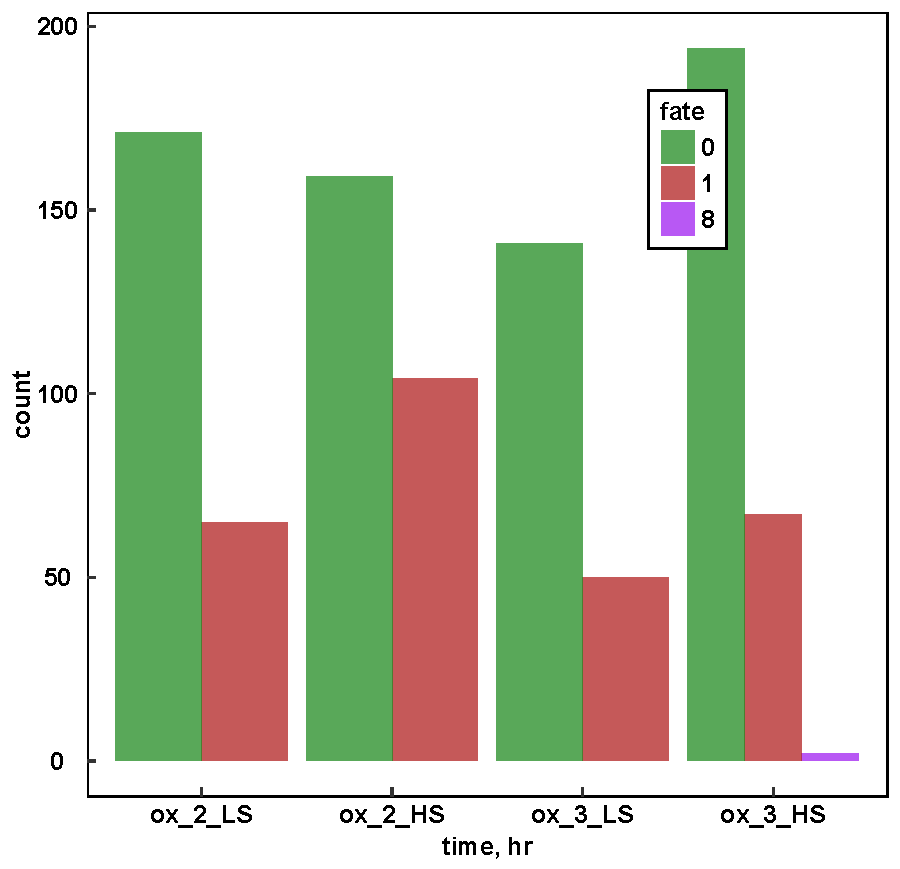
\includegraphics[width=.6\linewidth]{img/fateBytype.pdf} 
%		\vspace{4ex}
	\end{minipage}%% 
	\begin{minipage}[b]{0.5\linewidth}
		\centering
		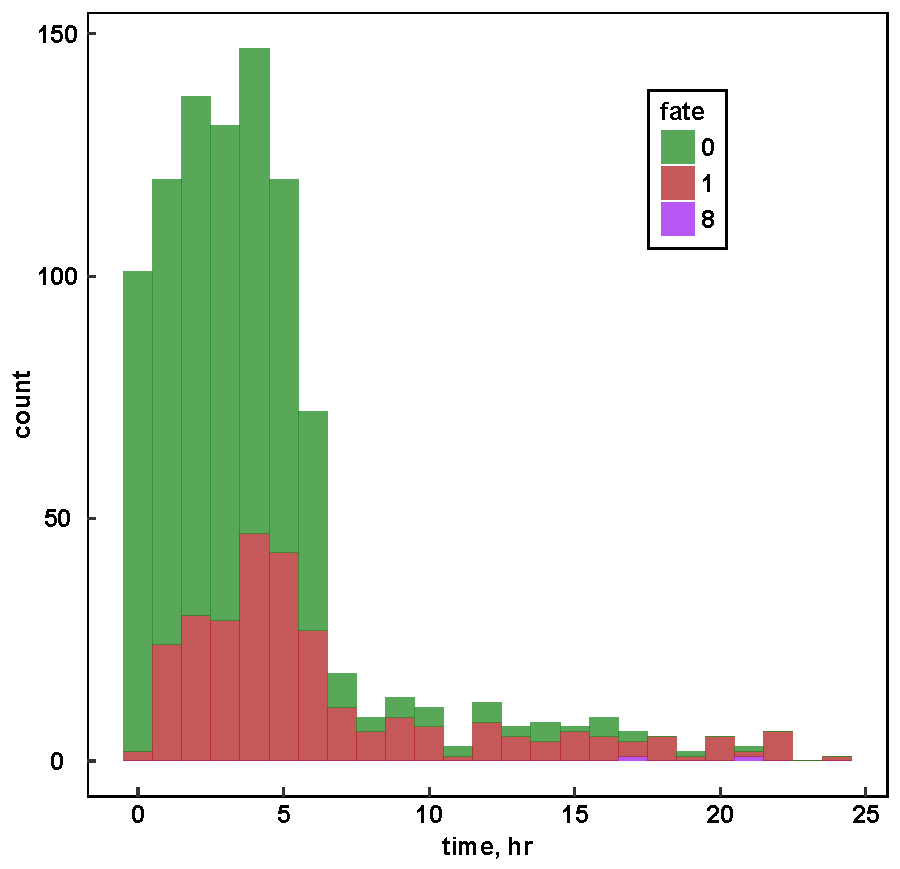
\includegraphics[width=.6\linewidth]{img/timeByfate.pdf} 
%		\vspace{4ex}
	\end{minipage} 
\end{figure}
\end{frame}


\begin{frame}
\begin{itemize}
\item 0: [NH3], [N]\#[N], [C+]\#[O-], [C+]\#[NH-], [N]\#[CH]
\item 1: [CH+]=[CH3-], [NH]=[O], [CH+]=[OH-], [CH2+]-[OH2-]
\item 8: [OH2-]-[PH+], [P+]=[OH-], [PH+]-[OH2-], [NH2-]=[CH+]
\end{itemize}
\end{frame}


% % % % % % % % % % % % % % % %
%backup of the setsizes and entropies for individual mono/bi split sets
% % % % % % % % % % % % % % % %
%\begin{frame}
%\frametitle{Monodentate Sets}
%The sizes of the subsets of the monodentate octahedral space.
%\begin{table}[]
%	\centering
%%	\caption{The sizes of the subsets of the monodentate octahedral space.}
%	\label{tab:space-sizes-mono}
%	\begin{tabular}{llcr}
%		\toprule
%		Set 					& description		       & formula					        	   & size \\
%		\midrule
%		Homoleptics             & eq = ax                  & $\frac{405!}{404! \cdot  1!}$           & 405        \\[0.1cm]
%		"5+1" symmetric         & eq = ax1 $\neq$ ax2      & $\frac{405!}{403! \cdot  1! \cdot  1!}$ & 163,620    \\[0.1cm]
%		Strongly symmetric      & eq $\neq$ ax             & $\frac{405!}{403! \cdot  1! \cdot  1!}$ & 163,620    \\[0.1cm]
%		"4+2" symmetric         & eq1 $\neq$ eq2 = ax      & $\frac{405!}{403! \cdot  1! \cdot 1!}$  & 163,620    \\[0.1cm]
%		Equatorially asymmetric & eq1 $\neq$ eq2 $\neq$ ax & $\frac{405!}{402! \cdot  3!}$           & 10,989,810 \\[0.1cm]
%		Weakly symmetric        & eq $\neq$ ax1 $\neq$ ax2 & $\frac{405!}{402! \cdot  2! \cdot  1!}$ & 32,969,430 \\[0.1cm]
%		Complete Heteroleptics  & $L_i \neq L_j$           & $\frac{405!}{399! \cdot  6!}$           & $\approx 5.9 \cdot 10^{12}$ \\[0.1cm]
%		Octahedral Space        & all                      & $405^6                      $           & $\approx 4.4 \cdot 10^{15}$ \\
%		\bottomrule
%	\end{tabular}
%	\end{table}
%\end{frame}
%
%\begin{frame}
%	\frametitle{Bidentate Sets}
%	The sizes of the subsets of the bidentate octahedral space.
%	
%	\begin{table}[]
%	\centering
%%	\caption{The sizes of the subsets of the bidentate octahedral space.}
%	\label{tab:space-sizes-bi}
%	\begin{tabular}{llcr}
%		\toprule
%		Set 					& description		       & formula					        	 & size \\
%		\midrule
%		Homoleptics             & eq = ax                  & $\frac{148!}{147! \cdot  1!}$           & 148        \\[0.1cm]
%		Strongly symmetric AC   & eq $\neq$ ax             & $\frac{148!}{146! \cdot  1! \cdot  1!}$ & 21,756    \\[0.1cm]
%		Strongly symmetric ADC  & eq $\neq$ ax             & $405 \cdot  148$                        & 59,940    \\[0.1cm]
%		"4+2" symmetric         & eq1 $\neq$ eq2 = ax      & $\frac{148!}{146! \cdot  1! \cdot 1!}$  & 21,756    \\[0.1cm]
%		Equatorially asymmetric AC & eq1 $\neq$ eq2 $\neq$ ax & $\frac{148!}{145! \cdot  3!}$        & 529,396 \\[0.1cm]
%		Equatorially asymmetric ADC& eq1 $\neq$ eq2 $\neq$ ax & $\frac{405 \cdot 148!}{146! \cdot  2!}$& 4,405,590 \\[0.1cm]
%		Weakly symmetric        & eq $\neq$ ax1 $\neq$ ax2 & $\frac{405! \cdot 148}{403! \cdot  2!}$ & 12,107,880 \\[0.1cm]
%		\bottomrule
%	\end{tabular}
%	\end{table}
%\end{frame}
%
%\begin{frame}
%\frametitle{Monodentate Footprints}
%	\begin{table}[]
%	\centering
%	\caption{Entropic footprint}
%	\label{tab:ent-footprint}
%	\begin{tabular}{lcr}
%		\toprule
%		Set 					    &  $H_{\textrm{KDE}}^{\textrm{monodent}}$   & $H_{\textrm{KDE}}^{\textrm{bident}}]$ \\
%		\midrule
%		Homoleptics                 &  19.7  & 15.63   \\[0.1cm]
%		"5+1" symmetric             &  13.7  & -       \\[0.1cm]
%		Strongly symmetric AC       &  -     & 9.47    \\[0.1cm]
%		Strongly symmetric ADC      &  12.70 & 5.53    \\[0.1cm]
%		"4+2" symmetric             &  12.70 & 9.47    \\[0.1cm] 
%		Weakly symmetric            &  8.1   & 7.70    \\[0.1cm]
%		Equatorially asymmetric AC  &  -     & 10.04   \\[0.1cm]
%		Equatorially asymmetric ADC &        &         \\[0.1cm]
%
%		\bottomrule
%	\end{tabular}
%	\end{table}
%\end{frame}


\end{document}